%%% Template originaly created by Karol Kozioł (mail@karol-koziol.net) and modified for ShareLaTeX use

\documentclass[a4paper,11pt]{article}

\usepackage[T1]{fontenc}
\usepackage[utf8]{inputenc}
\usepackage{graphicx}
\graphicspath{ {./images/} }

\usepackage{xcolor}

\renewcommand\familydefault{\sfdefault}
\usepackage{tgheros}

\usepackage{amsmath,amssymb,amsthm,textcomp,latexsym}
\usepackage{enumerate}
\usepackage{multicol}
\usepackage{tikz}

\usepackage{caption}
\usepackage{subcaption}
\usepackage{epstopdf}
\usepackage{cancel}


\usepackage{geometry}
\geometry{total={210mm,297mm},
left=25mm,right=25mm,%
bindingoffset=0mm, top=20mm,bottom=20mm}


\linespread{1.3}

\newcommand{\linia}{\rule{\linewidth}{0.5pt}}

% custom theorems if needed
\newtheoremstyle{mytheor}
    {1ex}{1ex}{\normalfont}{0pt}{\scshape}{.}{1ex}
    {{\thmname{#1 }}{\thmnumber{#2}}{\thmnote{ (#3)}}}

\theoremstyle{mytheor}
\newtheorem{defi}{Definition}

% my own titles
\makeatletter
\renewcommand{\maketitle}{
\begin{center}
\vspace{2ex}
{\huge \textsc{\@title}}
\vspace{1ex}
\\
\linia\\
\@author \hfill \@date
\vspace{4ex}
\end{center}
}
\makeatother
%%%

% custom footers and headers
\usepackage{fancyhdr}
\pagestyle{fancy}
\lhead{Projeto 1}
\chead{}
\rhead{2019.2}
\lfoot{}
\cfoot{}
\rfoot{Page \thepage}
\renewcommand{\headrulewidth}{0pt}
\renewcommand{\footrulewidth}{0pt}
%

% code listing settings
\usepackage{listings}
\lstset{
    language=Matlab,
    basicstyle=\ttfamily\small,
    aboveskip={1.0\baselineskip},
    belowskip={1.0\baselineskip},
    columns=fixed,
    extendedchars=true,
    breaklines=true,
    tabsize=4,
    prebreak=\raisebox{0ex}[0ex][0ex]{\ensuremath{\hookleftarrow}},
    frame=lines,
    showtabs=false,
    showspaces=false,
    showstringspaces=false,
    keywordstyle=\color[rgb]{0.627,0.126,0.941},
    commentstyle=\color[rgb]{0.133,0.545,0.133},
    stringstyle=\color[rgb]{01,0,0},
    numbers=left,
    numberstyle=\small,
    stepnumber=1,
    numbersep=10pt,
    captionpos=t,
    escapeinside={\%*}{*)}
}

%%%----------%%%----------%%%----------%%%----------%%%

\begin{document}

\title{Robótica e Automação}

\author{Raphael Barros Parreira}

\date{}

\maketitle

\section*{Questão 1}


A figura \ref{fig:kgen3_representacao_poe} mostra a representação do manipulador Kinova Gen3 usando o método do Enfoque de Exponenciais. Os eixos de rotação estão na mesma direção e sentido dos eixos $ Z $ em cada origem.

A figura \ref{fig:ex1_configuracoes} mostra a validação do modelo de Cinemática Direta achado. As três configurações (A, B e C) podem ser vistas na tabela \ref{tab:ex1_configuracoes}. A função usada para desenhar o manipulador é a \textit{showarm()}, disponibilizada pelo professor no \textit{Moodle} da Poli.


\begin{figure}[!ht]
\centering
\caption{Representação do Enfoque de Exponencias do Manipulador Kinova Gen3.}
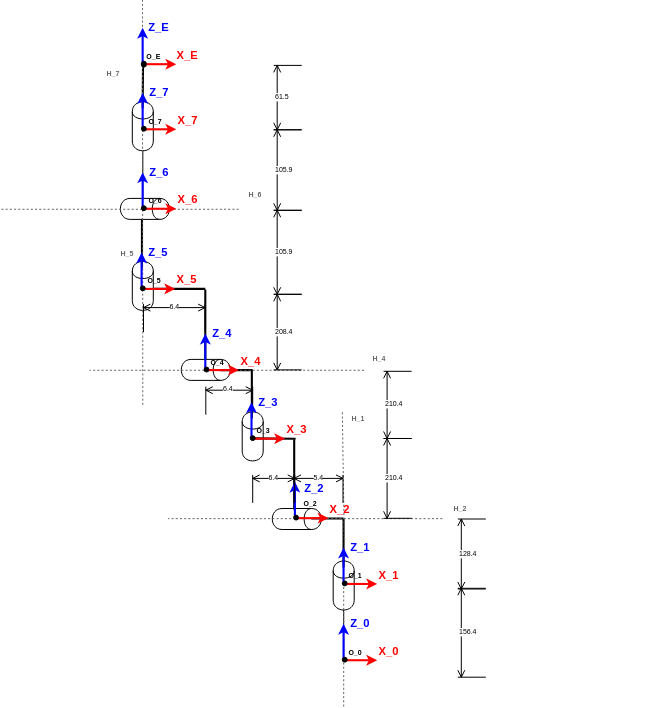
\includegraphics[scale=1]{figs/ex1_poe}
\label{fig:kgen3_representacao_poe}
\end{figure}

\begin{gather*}
\vec{h}_1 = \vec{z} \quad
\vec{h}_2 = \vec{x} \quad
\vec{h}_3 = \vec{z} \quad
\vec{h}_4 = \vec{x} \quad
\vec{h}_5 = \vec{z} \quad
\vec{h}_6 = \vec{x} \quad
\vec{h}_7 = \vec{z}
\\
R_{01} = e^{\vec{h}_1\theta_1} = e^{\widehat{z}\theta_1} \quad
R_{12} = e^{\vec{h}_2\theta_2} = e^{\widehat{x}\theta_2} \quad
R_{23} = e^{\vec{h}_3\theta_3} = e^{\widehat{z}\theta_3} \\
R_{34} = e^{\vec{h}_4\theta_4} = e^{\widehat{x}\theta_4} \quad
R_{45} = e^{\vec{h}_5\theta_5} = e^{\widehat{z}\theta_5} \quad
R_{56} = e^{\vec{h}_6\theta_6} = e^{\widehat{x}\theta_6} \quad
R_{67} = e^{\vec{h}_7\theta_7} = e^{\widehat{z}\theta_7}
\\
\vec{p}_{01} = l_0\vec{z}_0 \quad
\vec{p}_{12} = l_{1z}\vec{z}_1 - l_{1x}\vec{x}_1 \quad
\vec{p}_{23} = l_{2z}\vec{z}_2 - l_{2x}\vec{x}_2 \quad
\vec{p}_{34} = l_{3z}\vec{z}_3 - l_{3x}\vec{x}_3 \\
\vec{p}_{45} = l_{4z}\vec{z}_4 - l_{4x}\vec{x}_4 \quad
\vec{p}_{56} = l_5\vec{z}_5 \quad
\vec{p}_{67} = l_6\vec{z}_6 \quad
\vec{p}_{7e} = l_7\vec{z}_7
\\
T_{0e} = T_{01}T_{12}T_{23}T_{34}T_{45}T_{56}T_{67}T_{7e}
\end{gather*}

\begin{table}[!ht]
\centering
\caption{Dimensões dos elos da representação do manipulador Kinova Gen3 (figura \ref{fig:kgen3_representacao_poe})}
\label{tab:kgen3_representacao_dim}

\begin{tabular}{|c|c|c|c|c|c|c|c|c|c|c|c|c|}
\hline
             & $l_0$ & $l_{1x}$ & $l_{1z}$ & $l_{2x}$ & $l_{2z}$ & $l_{3x}$ & $l_{3z}$ & $l_{4x}$ & $l_{4z}$ \\ \hline
Dimensão (m) & 0.1564 & 0.1284 & 0.0054 & 0.2104 & 0.0054 & 0.2104 & 0.0064 & 0.2084 & 0.0064  \\ \hline
\end{tabular}
\begin{tabular}{|c|c|c|c|}
\hline
             & $l_5$ & $l_6$ & $l_7$ \\ \hline
Dimensão (m) & 0.1059 & 0.1059 & 0.0615 \\ \hline
\end{tabular}
\end{table}

\begin{table}[!ht]
\centering
\caption{Configurações do manipulador Kinova Gen3}
\label{tab:ex1_configuracoes}
\begin{tabular}{|c|c|c|c|}
\hline
Configuração & A & B & C  \\ \hline
$\theta_1$ & $0$ & $0$ & $0$ \\ \hline
$\theta_2$ & $0$ & $-\pi/2$ & $-\pi/2$ \\ \hline
$\theta_3$ & $0$ & $0$ & $0$ \\ \hline
$\theta_4$ & $0$ & $0$ & $\pi/2$ \\ \hline
$\theta_5$ & $0$ & $\pi/2$ & $0$ \\ \hline
$\theta_6$ & $0$ & $\pi/2$ & $0$ \\ \hline
$\theta_7$ & $0$ & $0$ & $0$ \\ \hline
\end{tabular}
\end{table}

\begin{figure}[!ht]
\centering
  \begin{minipage}{\linewidth}
  \centering
    \begin{subfigure}[b]{0.45\textwidth}
    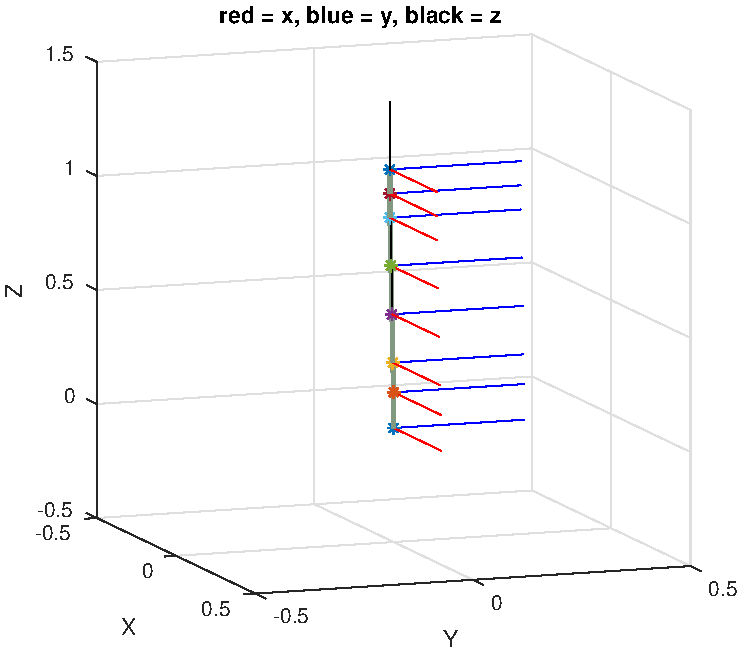
\includegraphics[width=1\textwidth]{figs/ex1_a.pdf}
    \caption{Configuração A}
    \end{subfigure}
    \begin{subfigure}[b]{0.45\textwidth}
    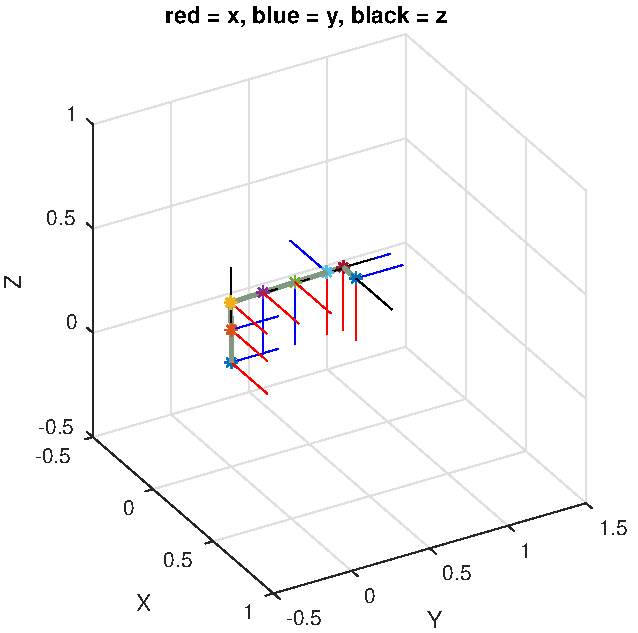
\includegraphics[width=1\textwidth]{figs/ex1_b.pdf}
    \caption{Configuração B}
    \end{subfigure}
  \end{minipage}
  \begin{minipage}{\linewidth}
  \centering
    \begin{subfigure}[b]{0.45\textwidth}
    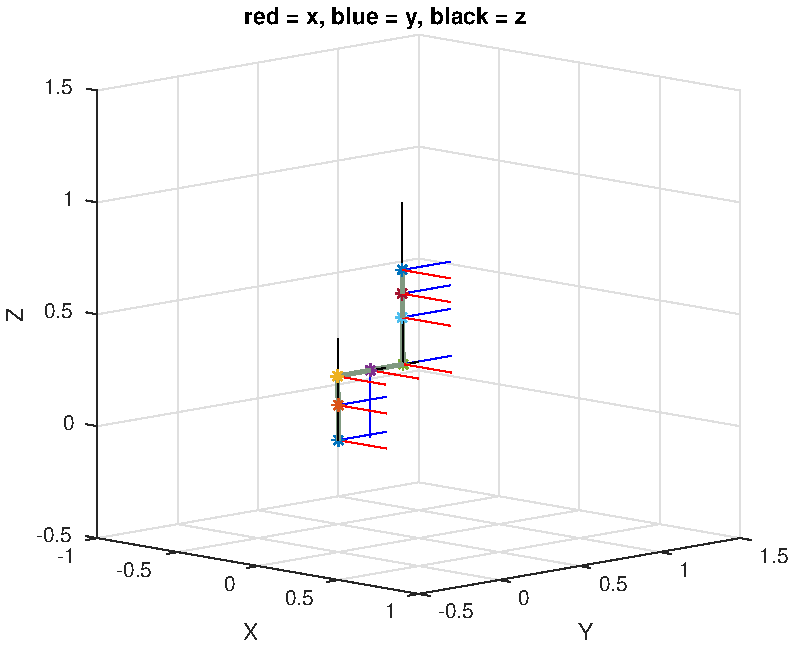
\includegraphics[width=1\textwidth]{figs/ex1_c.pdf}
    \caption{Configuração C}
    \end{subfigure}
  \end{minipage}
\caption{Representação do manipulador Kinova Gen3 no Enfoque de Exponenciais nas configurações A, B e C (tabela \ref{tab:ex1_configuracoes})}
\label{fig:ex1_configuracoes}
\end{figure}



\section*{Questão 2}

A figura \ref{fig:kgen3_representacao_dh} mostra a representação do Manipulador pelo método de Denavit-Hartenberg Standard. A tabela \ref{tab:ex2_param_tabela_dh} exibe os parâmetros encontrados para o método.

\begin{figure}[!ht]
\centering
\caption{Representação do Denavit-Hartenberg Standard do Manipulador Kinova Gen3.}
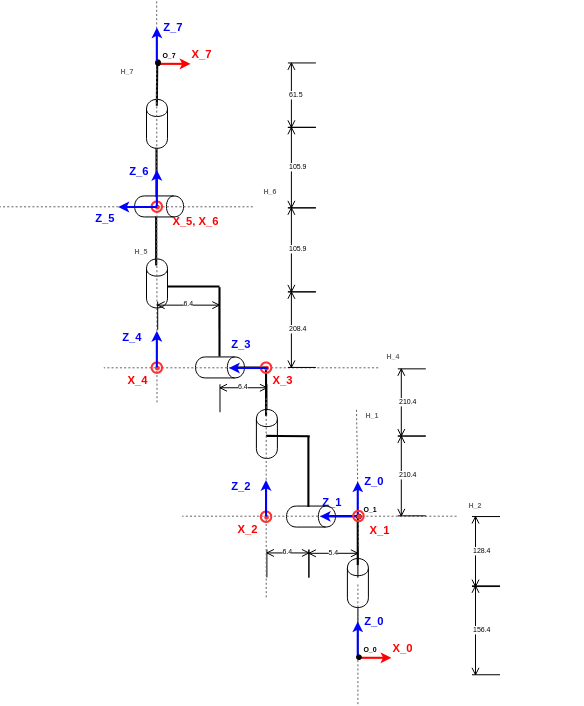
\includegraphics[scale=1]{figs/ex2_dh}
\label{fig:kgen3_representacao_dh}
\end{figure}


\begin{table}[!ht]
\centering
\caption{Tabela Denavit Hartenberg Standard para o Manipulador}
\label{tab:ex2_param_tabela_dh}
\begin{tabular}{|c|c|c|c|c|c|c|}
\hline
\textbf{Elo i} & \textbf{$\theta_i$} & \textbf{$d_i$} & \textbf{$a_i$} & \textbf{$\alpha_i$} & \textbf{type} & \textbf{offset} \\ \hline
1                & $\theta_1$            & $l_{0} + l_{1z}$     & $0$         & $\pi/2$               & $0$             & $-\pi/2$           \\ \hline
2                & $\theta_2$            & $l_{2x} + l_{3x}$    & $0$         & $-\pi/2$              & $0$             & $0$           \\ \hline
3                & $\theta_3$            & $l_{2z} + l_{3z}$    & $0$         & $\pi/2$               & $0$             & $0$               \\ \hline
4                & $\theta_4$            & $l_{3x} + l_{4x}$    & $0$         & $-\pi/2$              & $0$             & $0$               \\ \hline
5                & $\theta_5$            & $l_{4z} + l_{5}$     & $0$         & $\pi/2$               & $0$             & $0$               \\ \hline
6                & $\theta_6$            & $0$                  & $0$         & $-\pi/2$              & $0$             & $0$           \\ \hline
7                & $\theta_7$            & $l_6+l_7$            & $0$         & $0$                   & $0$             & $\pi/2$           \\ \hline
\end{tabular}
\end{table}



\section*{Questão 3}

O item $a$ da figura \ref{fig:ex4_configuracoes} exibe o modelo gerado pela classe SerialLink do Robot Toolbox. O manipulador se encontra na posição zero.

\section*{Questão 4}

A figura \ref{fig:ex4_configuracoes} exibe as três configurações usadas presentes na tabela \ref{tab:ex1_configuracoes}.

\begin{figure}[!ht]
\centering
  \begin{minipage}{\linewidth}
  \centering
    \begin{subfigure}[b]{0.45\textwidth}
    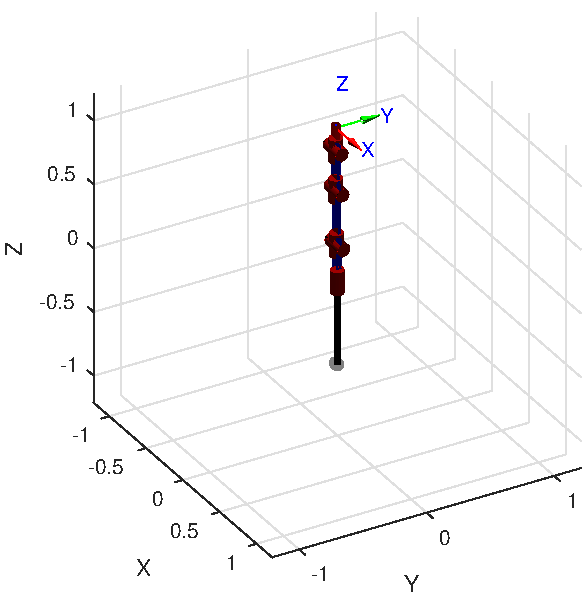
\includegraphics[width=1\textwidth]{figs/ex4_a.pdf}
    \caption{Configuração A}
    \end{subfigure}
    \begin{subfigure}[b]{0.45\textwidth}
    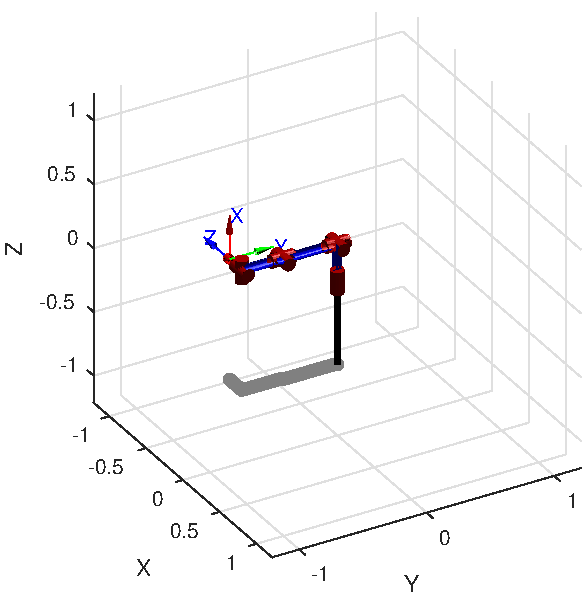
\includegraphics[width=1\textwidth]{figs/ex4_b.pdf}
    \caption{Configuração B}
    \end{subfigure}
  \end{minipage}
  \begin{minipage}{\linewidth}
  \centering
    \begin{subfigure}[b]{0.45\textwidth}
    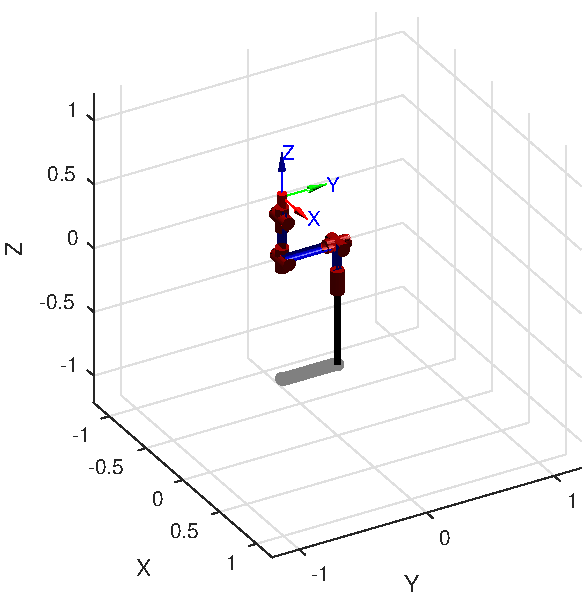
\includegraphics[width=1\textwidth]{figs/ex4_c.pdf}
    \caption{Configuração C}
    \end{subfigure}
  \end{minipage}
\caption{Representação do manipulador no Denavit Hartenberg Standard nas configurações A, B e C (tabela \ref{tab:ex1_configuracoes})}
\label{fig:ex4_configuracoes}
\end{figure}


\section*{Questão 5}

Para se fazer a Cinemática Inversa é necessário escolher uma posição $p_{be} $ e uma orientação $R_{Be}$ finais do manipulador, e uma configuração inicial do manipulador. A posição zero no manipulador é uma região de singularidade. Portanto, para que a função \textit{ikine()} convirja, é necessário mudar a configuração inicial. 

A tabela \ref{tab:ex5_ikine_configuracao} exibe os ângulos das juntas escolhidos e os encontrados. A figura \ref{fig:ex5_configuracoes} mostra o manipulador com as duas configurações.


\begin{gather}
\label{eq:ex5_tbe}
T_{be} = \begin{bmatrix} R_{be} & p_{be} \\ 0 & 1 \end{bmatrix}
\\ 
\label{eq:ex5_rbe}
R_{be} = \begin{bmatrix} 0 & 0 & 1 \\ 0 & -1 & 0 \\ 1 & 0 & 0 \end{bmatrix}
\qquad
p_{be} = \begin{bmatrix} 0.7 \\ 0 \\ 0.4 \end{bmatrix}
\end{gather}

\begin{table}[!ht]
\centering
\caption{Configuração inicial para a função ikine.}
\label{tab:ex5_ikine_configuracao}

\begin{tabular}{|c|c|c|c|c|c|c|c|}
\hline
Juntas  & $\theta_1$ & $\theta_2$ & $\theta_3$ & $\theta_4$ & $\theta_5$ & $\theta_6$ & $\theta_7$ \\ \hline
Inicial     & 0 & $-\pi /2$ & 0 & 0 & 0 & 0 & 0 \\ \hline
Resultante     & 1.1630 & -0.8868 & 0.8339 & -1.4722 & 0.2492 & 0.7224 & 0.7613 \\ \hline
\end{tabular}
\end{table}


\begin{figure}[!ht]
\centering
  \begin{minipage}{\linewidth}
  \centering
    \begin{subfigure}[b]{0.45\textwidth}
    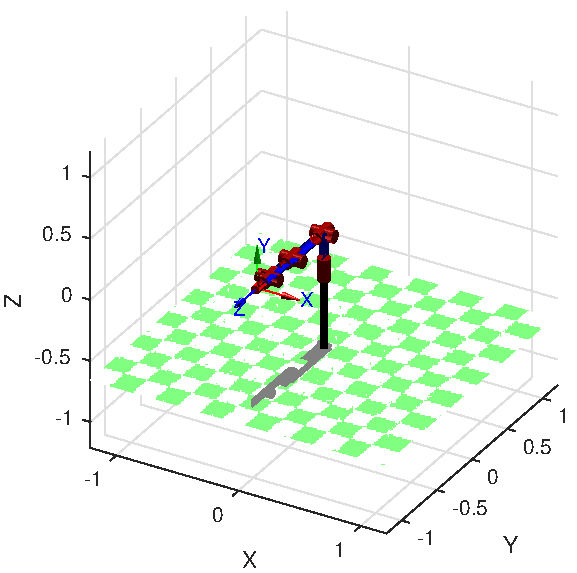
\includegraphics[width=1\textwidth]{figs/ex5_inicial.pdf}
    \caption{Inicial}
    \end{subfigure}
    \begin{subfigure}[b]{0.45\textwidth}
    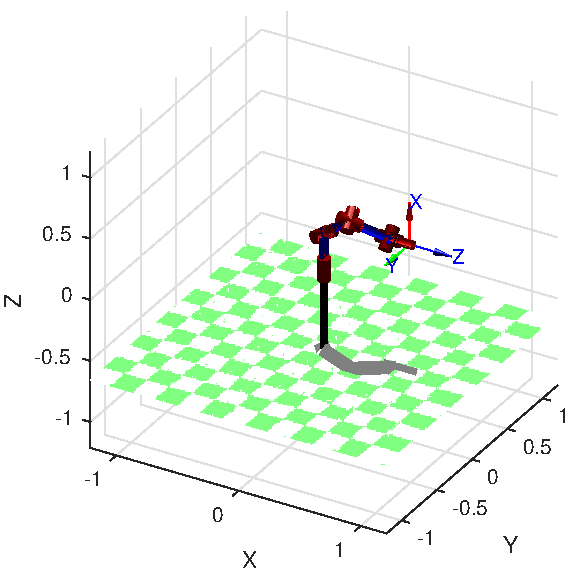
\includegraphics[width=1\textwidth]{figs/ex5_resposta.pdf}
    \caption{Resultante}
    \end{subfigure}
  \end{minipage}
\caption{Representações do manipulador nas configurações inicial e na resultante. (tabela \ref{tab:ex5_ikine_configuracao})}
\label{fig:ex5_configuracoes}
\end{figure}



\section*{Questão 6}

\begin{gather*}
J_7 = \begin{bmatrix} 
\vec{h}_1 \times \vec{p}_{17} & \vec{h}_2 \times \vec{p}_{27} & \vec{h}_3 \times \vec{p}_{37} & \vec{h}_4 \times \vec{p}_{47} & \vec{h}_5 \times \vec{p}_{57} & \vec{h}_6 \times \vec{p}_{67} & \vec{h}_7 \times \vec{p}_{77} \\
\vec{h}_1 & \vec{h}_2 & \vec{h}_3 & \vec{h}_4 & \vec{h}_5 & \vec{h}_6 & \vec{h}_7 \end{bmatrix}
\end{gather*}

\begin{equation*}
\begin{aligned}
(J_7)_0 &= 
\left[\begin{matrix} 
(\vec{h}_1)_0 \times (\vec{p}_{17})_0 & (\vec{h}_2)_0 \times (\vec{p}_{27})_0 & (\vec{h}_3)_0 \times (\vec{p}_{37})_0 & (\vec{h}_4)_0 \times (\vec{p}_{47})_0 \\
(\vec{h}_1)_0 & (\vec{h}_2)_0 & (\vec{h}_3)_0 & (\vec{h}_4)_0
\end{matrix}\right. \\
&\qquad\qquad
\left.\begin{matrix}
(\vec{h}_5)_0 \times (\vec{p}_{57})_0 & (\vec{h}_6)_0 \times (\vec{p}_{67})_0 & (\vec{h}_7)_0 \times (\vec{p}_{77})_0 \\
(\vec{h}_5)_0 & (\vec{h}_6)_0 & (\vec{h}_7)_0
\end{matrix}\right]
\end{aligned}
\end{equation*}


\section*{Questão 7}

\end{document}
